\documentclass[11pt,a4paper]{article}

\usepackage[utf8]{inputenc}
\usepackage[T1]{fontenc}
\usepackage{lmodern}        % T1 fonts with proper Unicode glyph mapping
\usepackage{cmap}           % embed ToUnicode CMaps -> text is copyable/searchable
\usepackage[margin=2.4cm]{geometry}
\usepackage{graphicx}
\usepackage{float}          % [H] to pin a figure exactly where it is written
\usepackage{booktabs}
\usepackage{amsmath}
\usepackage[strings]{underscore}

% Map font glyphs (incl. ff/fi/fl ligatures) to Unicode so extracted text is correct.
\input{glyphtounicode}
\pdfgentounicode=1

\title{Sensitivity analysis of the \texttt{remote\_share} parameter\\
       \large An agent-based model of a software development team}
\author{Miłosz Lewandowski}
\date{}

\begin{document}
\maketitle
\vspace{-1.5em}

\noindent
This report studies how one parameter, \texttt{remote\_share}, affects an agent-based model of a
ten-person software team. The parameter is the chance that a developer works from home on a given
day. Only this parameter is changed; all others keep their default values. Each simulation covers
one year (24 sprints) with learning and turnover switched on. The parameter is swept over its full
range, from $0$ to $1$, in steps of $0.05$, with 80 repetitions at each level. A separate study with
400 repetitions at three levels is used to check how many repetitions are needed. The experiment and
the figures are produced by \texttt{sensitivity\_remote.py} and \texttt{plot\_sensitivity.py}.

\section{Experimental design}

Each run records four macroscopic quantities. \texttt{total\_velocity} is the number of story points
delivered during the year, and it is the main outcome. \texttt{avg\_wait} is the average number of
ticks a blocked developer waits for help, and it shows the small-scale mechanism that remote work
affects. \texttt{mean\_skill} and \texttt{attrition\_count} follow the two slower parts of the model,
the team's skill and the people who leave.

The range of the study is set by the parameter itself. Because \texttt{remote\_share} is a
probability, the interval $[0,1]$ is its only possible range, so there is no doubt about where to
start or stop. The number of repetitions needed is not the same for every quantity
(Figure~\ref{fig:conv}). A full year averages over many thousands of small events, so the mean of
\texttt{total\_velocity} settles quickly: about 40 repetitions already give it to within $\pm0.1\%$,
and 80 give $\pm0.08\%$ even at the noisiest end of the range. A count of rare events behaves very
differently. \texttt{attrition\_count} has a mean of about $1.1$ and a standard deviation of about
$1.0$, so its relative error is still near $\pm20\%$ at 80 repetitions and about $\pm9\%$ at 400.
Eighty repetitions are therefore more than enough for the throughput results below, but a count like
attrition would need several hundred.

\begin{figure}[ht]
\centering
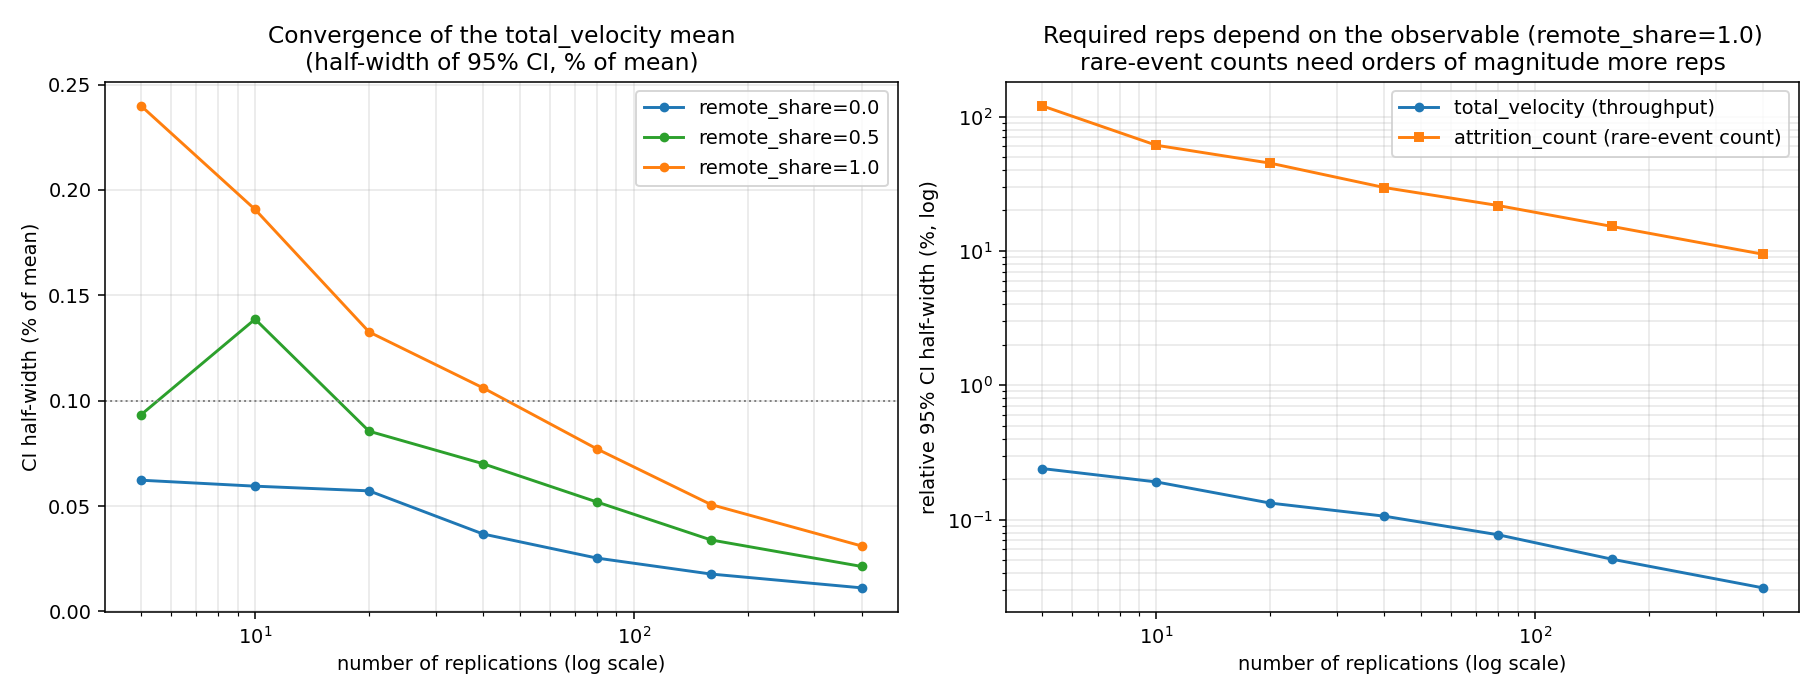
\includegraphics[width=0.80\textwidth]{sens_fig4_convergence.png}
\caption{Width of the 95\% confidence interval against the number of repetitions. Throughput (left)
settles quickly; the attrition count (right) needs far more runs to reach the same relative
precision.}
\label{fig:conv}
\end{figure}

\section{Results}

Throughput goes down as remote work increases, but only a little: by about $2.5\%$ between a fully
office-based and a fully remote team. The fall is smooth and steady, with no sudden jump
(Figure~\ref{fig:rel}, left). The mechanism behind it changes much more. The average wait per blocker
rises by $59\%$ (Figure~\ref{fig:rel}, right), because help that involves someone at home is
asynchronous and roughly five times slower than help in the office. A line showing the mean with a
confidence band is the natural way to present a single outcome against one continuous control; here
the band is thinner than the markers.

\begin{figure}[ht]
\centering
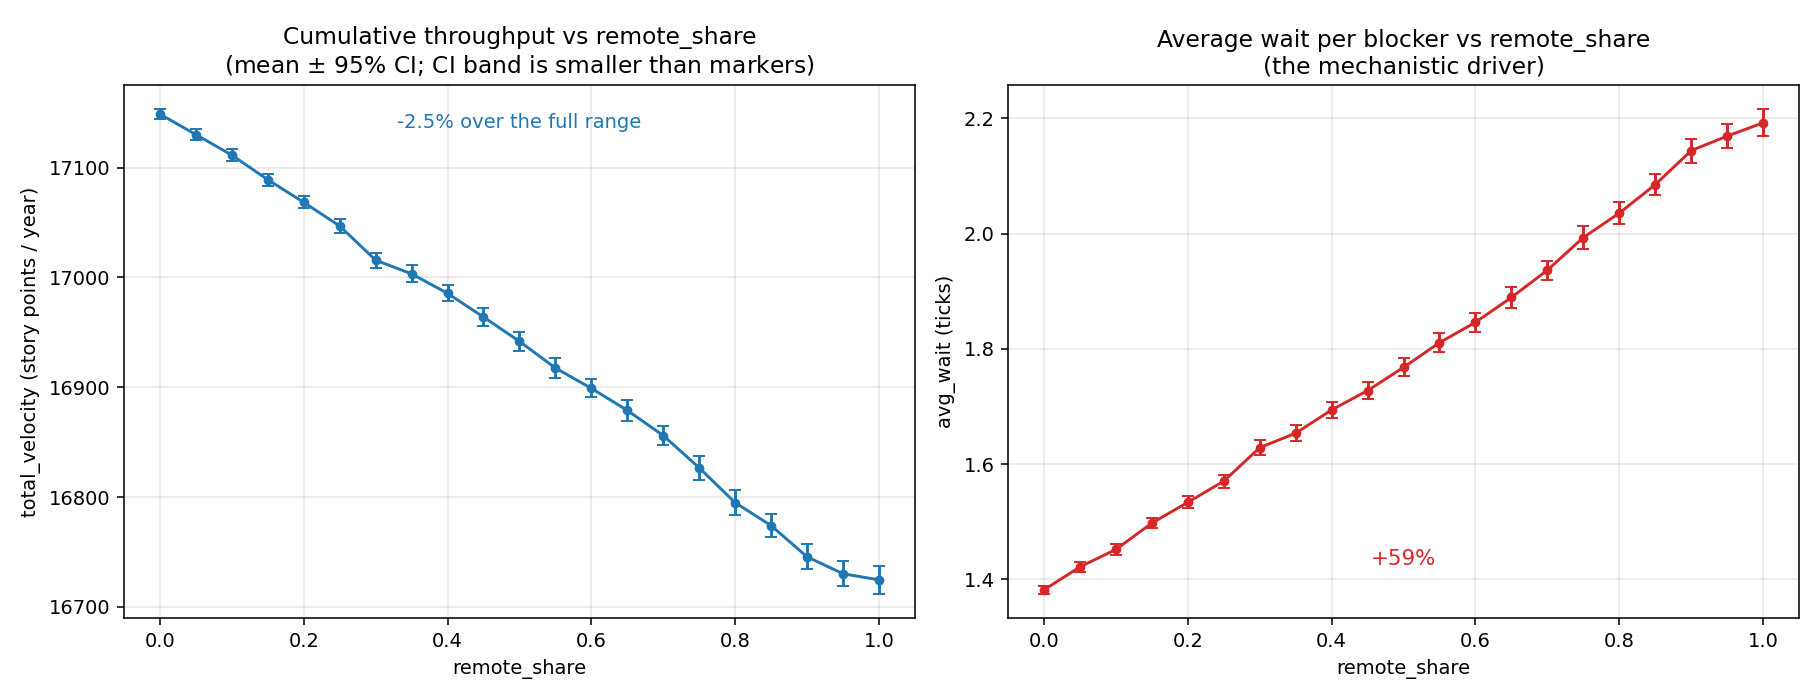
\includegraphics[width=0.80\textwidth]{sens_fig1_relationship.png}
\caption{Yearly throughput falls by $2.5\%$ across the full range (left), while the average wait per
blocker rises by $59\%$ (right). Means are shown with 95\% confidence intervals, 80 repetitions per
point.}
\label{fig:rel}
\end{figure}

Whether the mean is a good summary depends on the quantity. For \texttt{total\_velocity} it is: the
results of different runs lie close together and are roughly symmetric, with a coefficient of
variation between $0.1$ and $0.35\%$, so the mean and the median agree. For \texttt{attrition\_count}
it is not. That quantity is a small whole number, and between $29$ and $38\%$ of runs have zero
departures, so an average of $1.1$ matches almost no real run. In that case the distribution, or the
share of runs with no departures, describes the system better than the mean.

The mean curve also leaves out something the results should make clear: on its own it does not tell
the whole story. Figure~\ref{fig:disp} keeps the full set of run results instead of reducing each
level to a single average. The spread of yearly throughput grows clearly as remote work increases,
and the standard deviation roughly triples across the range, from about 20 to 59 story points, while
the mean moves by only $2.5\%$. So how predictable the output is depends on remote work much more
strongly than the average output does.

\begin{figure}[H]
\centering
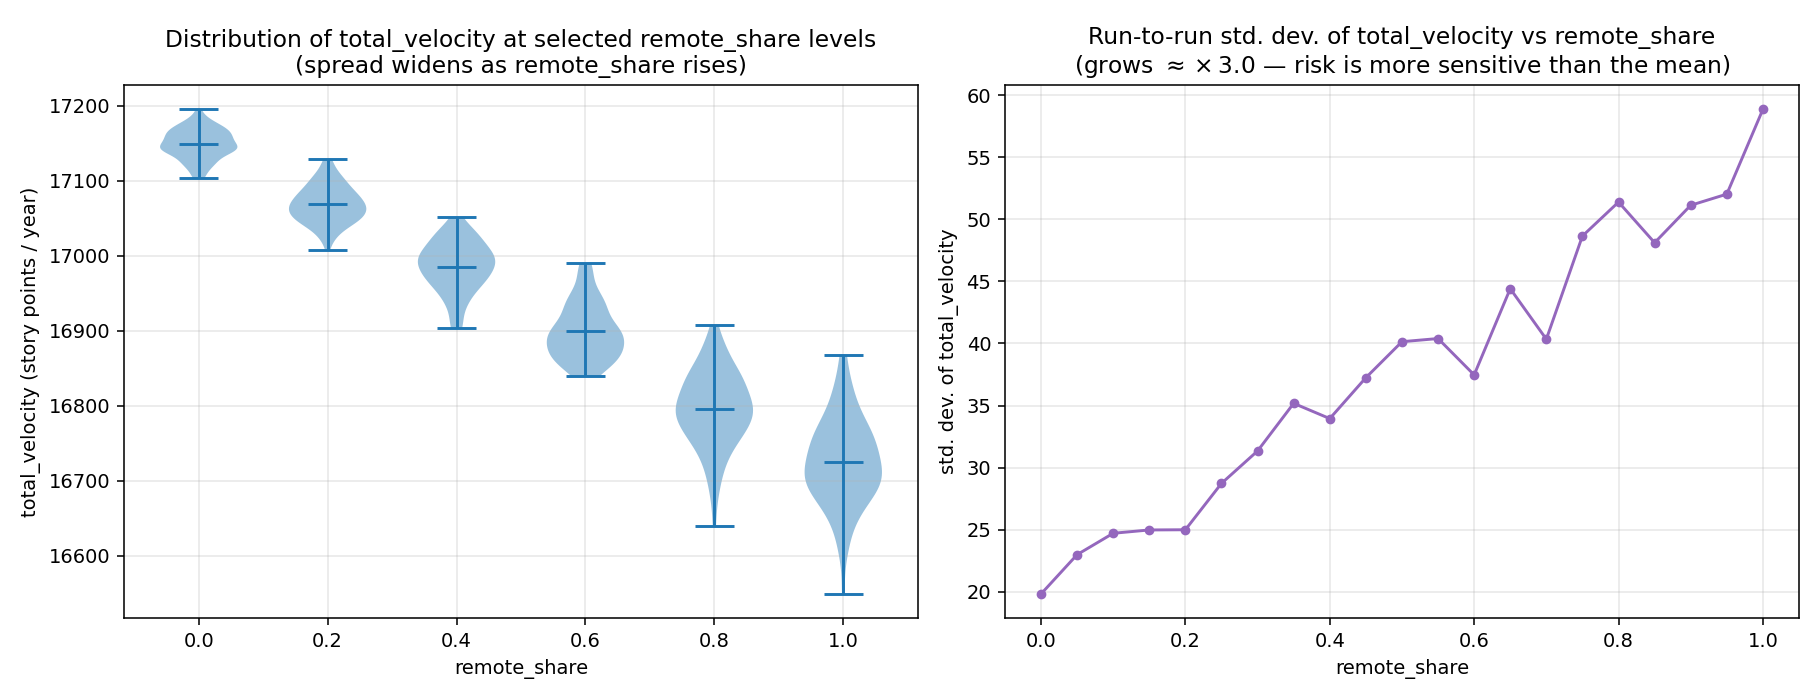
\includegraphics[width=0.80\textwidth]{sens_fig2_dispersion.png}
\caption{Spread of yearly throughput at each level (left) and its run-to-run standard deviation
(right). The mean barely changes, but the spread grows about threefold.}
\label{fig:disp}
\end{figure}

\section{Conclusions}

In numbers, more remote work makes the wait for help much longer ($+59\%$) but costs little
throughput ($-2.5\%$). In qualitative terms, the effect on throughput is gradual and steady, not a
collapse past some critical point.

Three findings deserve a closer look. First, a $59\%$ longer wait for help costs only $2.5\%$ of
throughput. The two are loosely linked because blockers are rare next to ordinary work. The extra
waiting adds up to about one thousand idle ticks, against roughly $77{,}000$ working ticks in the
year, which is close to $1.3\%$, the same order of magnitude as the drop we see. So the parameter
that looks most important in the mechanism is not the one that controls the final result.

Second, remote work does not reduce skill. The end-of-year \texttt{mean\_skill} stays flat across the
whole range, at about $0.88$. In the model, most learning comes from finishing tasks, which does not
depend on location. The extra mentoring value of in-office help applies only to the rarer cases of
resolving a blocker, so it has a small, second-order effect.

Third, the effect that matters most for a decision is on the spread, not on the mean. Moving to fully
remote work leaves the expected throughput almost the same but makes the year about three times less
predictable. An analysis that looked only at the average would miss this completely.

One flat result needs a caveat rather than a conclusion. \texttt{attrition\_count} shows no trend
with \texttt{remote\_share}, but only because the model links the two through a single coefficient,
\texttt{remote\_attrition\_coef}, whose default value is zero. With that setting, attrition simply
cannot respond. This link is a genuinely open empirical question, namely whether remote work helps
retention or instead causes isolation, and sweeping this coefficient over $[-1,1]$ is the natural
next step. Since a departure replaces a senior developer with a junior, even a moderate effect
through this channel would probably outweigh the $2.5\%$ throughput effect studied here, and, unlike
it, would carry over into the skill channel over several years.

\end{document}
